\documentclass{standalone}
\usepackage{tikz}
\usepackage{tabularx}
\usepackage{colortbl}
\usepackage{booktabs}

\begin{document}
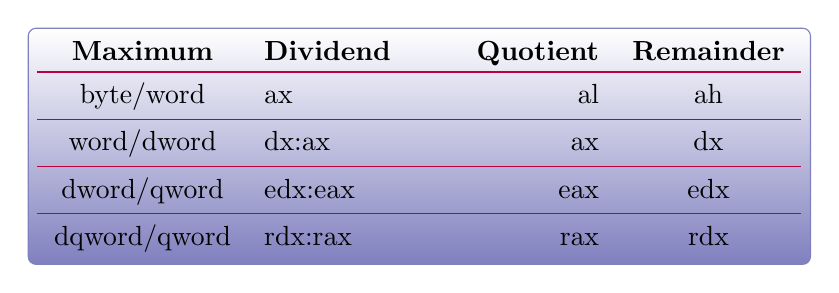
\begin{tikzpicture}[tab_style/.style={
		draw=blue!50!black!50,
		top color=white,
		bottom color=blue!50!black!50,
		rounded corners=1mm
	}]

\node[tab_style](tbl) {
\begin{tabularx}{.8\textwidth}{cXrcc}
\arrayrulecolor{purple}
\textbf{Maximum} & \textbf{Dividend} & \textbf{Quotient} & \textbf{Remainder} \\
\toprule
byte/word & ax & al & ah \\
\midrule
word/dword & dx:ax & ax & dx \\
\midrule
dword/qword & edx:eax & eax & edx \\
\midrule
dqword/qword & rdx:rax & rax & rdx 
\end{tabularx}
};

\end{tikzpicture}
\end{document}
